\documentclass{llncs}
\usepackage{amsmath,amssymb}
\usepackage{booktabs}
\usepackage{graphicx}
\usepackage[hidelinks]{hyperref}
\usepackage{enumitem}
\usepackage{caption}
\usepackage{subcaption}
\usepackage{tikz}
\usetikzlibrary{shapes.geometric, arrows.meta, positioning, fit, decorations.pathreplacing}

\begin{document}

\title{Access-Pattern Leakage in ML Training Pipelines: Measurement and ORAM-Based Mitigation}

\author{Caden Roberts}
\institute{University of California, Santa Cruz}

\maketitle

\begin{abstract}
Machine learning training pipelines expose structured data access patterns, including which samples are accessed, how often, and in what order.
These access patterns are observable at the storage layer---without access to model outputs, gradients, or parameters---and may provide signals for downstream inference under structured sampling or auxiliary knowledge.
Existing privacy mechanisms, such as federated learning and differential privacy, protect model updates but do not address this access-pattern exposure.

In this work, we study access-pattern leakage in standard deep learning pipelines and evaluate an oblivious RAM (ORAM)-backed data loading design that obfuscatedcates the mapping between logical samples and physical accesses.
We implement a file-backed ORAM layer integrated with the PyTorch data loader and evaluate its impact on both privacy exposure and system performance.

We demonstrate that per-sample access frequency alone provides a measurable signal for membership inference in the plaintext setting, achieving near-perfect separation (AUC $\approx$ 1.00) in a controlled setting where holdout samples are never accessed.
Under ORAM-backed data loading, this signal is not directly observable due to the lack of linkage between observed accesses and logical samples.

We further characterize the performance overhead of ORAM-backed training across dataset size, batch size, worker count, and storage backend, observing slowdowns of up to 180$\times$ under our experimental configuration.
Our results identify cryptographic tree traversal and serialization as dominant factors limiting performance, with storage backend optimization yielding bounded improvements.

These findings highlight access-pattern exposure as a distinct and previously under-addressed privacy channel in machine learning systems, and motivate the need for privacy-preserving data access mechanisms alongside existing model- and gradient-level protections.
\end{abstract}

\keywords{access-pattern leakage \and side-channel attacks \and machine learning systems \and oblivious RAM \and privacy-preserving machine learning \and data access privacy \and secure data pipelines}

%% ----------------------------------------------------------------
\section{Introduction}

Privacy-preserving machine learning has received significant attention through techniques such as federated learning~\cite{mcmahan2017} and differential privacy~\cite{dwork2006}.
These approaches protect \emph{data values} during training: federated learning keeps raw data on-device, and differential privacy bounds what can be inferred about individual records from model outputs.
However, neither technique addresses \emph{storage-level access-pattern leakage}: the sequence and frequency of storage block reads that a training pipeline generates can expose information about the underlying data, independent of whether the data itself is encrypted.

A machine learning training loop repeatedly reads samples from a dataset.
In standard PyTorch, the \texttt{DataLoader} fetches samples by index: each call to \texttt{\_\_getitem\_\_(i)} issues a memory or disk read at an address determined by sample index~$i$.
The sequence of indices accessed during training, and the frequency with which each index appears, constitutes an access pattern that is observable to any entity monitoring the storage layer: the operating system, the cloud hypervisor, a co-located tenant on shared hardware, or a compromised storage controller.

This attack surface has received limited attention in production ML pipelines.
Federated learning~\cite{mcmahan2017}, differential privacy~\cite{dwork2006}, and secure aggregation~\cite{bonawitz2017} protect data values and gradient statistics but do not address access-pattern exposure at the data loading layer.
This setting captures a distinct and previously under-explored attack surface in ML systems: an adversary with storage-level observability can infer properties about the training data without access to model outputs, gradients, or parameters.
Oblivious RAM (ORAM) is a cryptographic primitive that aims to make physical access patterns unlinkable to logical data accesses.
This paper characterizes the access-pattern exposure surface of standard training pipelines and evaluates Path ORAM as a countermeasure.

We distinguish between (i)~directly observable access metadata under the modeled setup (sample order, frequency, and count), (ii)~properties that may be inferred under structured sampling strategies or auxiliary knowledge (batch grouping, dataset-scale proxies), and (iii)~downstream privacy risks such as membership inference, for which we provide a simple empirical signal demonstration.

Our contributions are:

\begin{enumerate}[label=(\arabic*), nosep]
    \item A characterization of what a storage-level adversary can directly observe from training access patterns under the stated setup, and what may be inferable under structured sampling assumptions.
    \item A formalization of the threat model and exposure profile distinguishing what Path ORAM hides from what it leaks.
    \item An ORAM-backed PyTorch data-loading layer that interposes between the dataset and the training loop, including a mediated multi-worker loader design.
    \item An illustrative overhead decomposition identifying four multiplicative cost factors: I/O amplification, cryptographic cost, parallelism loss, and serialization overhead.
    \item An 8-phase controlled evaluation quantifying overhead across storage backend, worker count, block size, model architecture, dataset size, and batch size on CIFAR-10 with ResNet-18, ResNet-50, and EfficientNet-B0.
    \item Empirical evidence that plaintext training exposes the full per-epoch sample permutation while ORAM removes the direct linkage between observed physical accesses and logical samples.
\end{enumerate}

We focus on characterizing access-pattern exposure and system overhead.
We include a simple membership inference demonstration using access frequency (Section~\ref{sec:inference}), but do not evaluate comprehensive downstream attacks such as label recovery or attribute inference.

%% ----------------------------------------------------------------
\section{Background and Related Work}
\label{sec:related}

\subsubsection{Path ORAM.}
ORAM was introduced by Goldreich and Ostrovsky~\cite{goldreich1996} to hide software access patterns from an adversary observing memory.
Path ORAM~\cite{stefanov2013} organizes $N$ data blocks in a binary tree of height $h = \lceil \log_2 N \rceil$.
Each logical access (read or write) requires: (1)~reading $h$ encrypted blocks along a root-to-leaf path, (2)~decrypting blocks and locating the target, (3)~re-encrypting and writing back the path (eviction), and (4)~remapping the target block to a new random leaf.
The per-access bandwidth is $O(\log N)$ blocks.
For $N = 50{,}000$ samples, $h = 16$, yielding ${\sim}34$ block operations per sample access (read path + write-back) at 4\,KB per block.

\subsubsection{ORAM in secure computation and ML.}
ORAM has been applied to secure computation and inference~\cite{goldreich1996,stefanov2013}, and related work on private inference uses cryptographic techniques to protect model weights and inputs~\cite{tramer2019,juvekar2018}, but integration of ORAM into ML \emph{training} pipelines remains underexplored.
Cache-based side-channel attacks can leak DNN architectures from shared hardware~\cite{yan2020}, further motivating access-pattern protection.
Prior work on privacy-preserving ML---federated learning~\cite{mcmahan2017}, differential privacy~\cite{dwork2006}, secure aggregation~\cite{bonawitz2017}---protects data values or gradient statistics, not storage-level access patterns.
Our setting is orthogonal to prior work that relies on model outputs or microarchitectural signals: we assume an adversary with storage-level observability only.

\subsubsection{Secure enclaves.}
Secure enclaves (e.g., Intel SGX) protect memory confidentiality and integrity from the OS and hypervisor, but they do \emph{not} hide access patterns~\cite{xu2015}: an adversary observing the enclave's storage I/O still sees which blocks are read and in what order.
Systems such as Gramine~\cite{gramine2022} run training inside enclaves for memory protection; ORAM addresses the complementary threat of storage-level access-pattern leakage.
ORAM and enclaves are orthogonal: enclaves protect \emph{what} is in memory; ORAM hides \emph{which} blocks are accessed.

\subsubsection{ORAM data loaders and concurrent ORAM.}
OBLIVIATOR~\cite{mavrogiannakis2025} provides oblivious parallel operators for database joins in shared memory, not for ML data-loading.
SONIC~\cite{talur2026} proposes concurrent ORAM through coordinated position-map updates and parallel eviction, which could recover the multi-worker parallelism lost by single-threaded Path ORAM.
PyORAM~\cite{pyoram} provides the underlying Path ORAM implementation used in this work; our contribution is the \texttt{ORAMDataset} abstraction, serialization for variable-size samples, and integration into PyTorch's training loop.

%% ----------------------------------------------------------------
\section{Threat Model and Leakage Analysis}
\label{sec:threat}

\subsection{Access Patterns as a Side Channel}

Even if every sample is stored encrypted at rest, the access pattern itself is observable to any entity that can monitor the storage layer.
Under the modeled setup where logical samples map to stable storage locations, an adversary with storage-layer visibility can directly observe the training data's ordering and per-sample access frequency.
Under structured sampling strategies (stratified batching, curriculum learning, hard-example mining), higher-level properties such as batch grouping or class-level structure may be inferable given auxiliary knowledge about the sampling policy.
These observations may provide signal for downstream membership inference~\cite{shokri2017}, though we do not evaluate concrete membership-inference attacks in this work.

During training, access patterns expose information along several axes:

\begin{enumerate}[label=\textbf{(\alph*)}, nosep]
    \item \textbf{Sample selection order.}
    The DataLoader shuffles indices each epoch to produce a random permutation.
    An adversary observing the permutation learns which samples appear in the same mini-batch.
    Pipelines using stratified sampling, class-balanced batching, or curriculum-based ordering produce non-uniform permutations where batch composition may correlate with label or demographic attributes if the adversary has auxiliary knowledge about the sampling policy.

    \item \textbf{Per-sample access frequency.}
    Curriculum learning, hard-example mining, and data augmentation strategies cause certain samples to be accessed more frequently.
    An adversary counting per-index access frequency can observe which samples are re-accessed, potentially indicating model difficulty or data distribution properties.

    \item \textbf{Data-dependent branching.}
    Some pipelines conditionally skip or re-read samples based on loss values or gradient norms.
    The resulting access pattern may be correlated with private label information.

    \item \textbf{Dataset composition.}
    The total number of distinct indices accessed reveals the effective dataset size.
    In federated or multi-tenant settings, this exposes how much data a participant contributed.

    \item \textbf{Timing correlations.}
    Variable-length samples produce access-time variations that may be correlated with private attributes of the data.
\end{enumerate}

\subsection{Adversary Model}

We consider an honest-but-curious adversary with the following capabilities:
\begin{itemize}[nosep]
    \item Full visibility into the storage layer: every block read and write, including the physical address, timestamp, and block size.
    \item No access to plaintext data values (data is encrypted at rest with AES-CTR).
    \item No access to model outputs, gradients, or parameters.
    \item No ability to modify the training computation (passive adversary).
\end{itemize}

The adversary passively observes access events and does not interfere with training execution.
This threat model is realistic for cloud ML platforms where the storage backend is operated by the cloud provider or shared with other tenants.

\medskip
\noindent\textbf{Setup assumptions.}
The modeled setup assumes: (i)~a stable mapping between logical sample indices and storage locations, (ii)~storage-level observability of block-level access sequences, and (iii)~no additional obfuscatedcation from distributed storage, aggressive caching, or preprocessing layers that might alter the access-to-storage mapping.
These assumptions hold for the evaluated PyTorch configuration but may not generalize to all training environments.

\subsection{Adversary Observations}

Table~\ref{tab:access_patterns} distinguishes between directly observable properties and those that may be inferred under additional assumptions.

\begin{table}[t]
\centering
\small
\caption{Comparison of observable access metadata in plaintext and ORAM-backed training pipelines.}
\label{tab:access_patterns}
\begin{tabular}{@{}p{3.2cm}p{3.6cm}p{4.4cm}@{}}
\toprule
\textbf{Property} & \textbf{Plaintext} & \textbf{ORAM-backed} \\
\midrule

Logical sample identity &
Directly observable from storage access mapping &
Not directly observable; physical accesses are randomized and unlinkable to logical samples \\
\addlinespace

Access frequency (per sample) &
Directly observable &
Not directly observable; only total access count is visible \\
\addlinespace

Access order (per sample) &
Directly observable &
Not directly observable; access sequence is obfuscatedcated \\
\addlinespace

Batch composition &
Directly observable from grouped accesses &
Not directly observable; grouping structure is not preserved at the physical level \\
\addlinespace

Dataset size &
Observable via distinct accessed items &
Approximate upper bound observable via ORAM tree capacity \\
\addlinespace

Class-level structure &
May be inferred from access patterns under structured sampling or auxiliary knowledge &
Not directly observable; inference depends on external information \\
\addlinespace

Access timing &
Per-sample timing may be observable &
Fixed block size reduces some timing variation; residual timing channels may remain \\
\addlinespace

Read/write ratio &
Observable and may reflect training behavior &
Observable at aggregate level (logical semantics preserved) \\

\bottomrule
\end{tabular}
\end{table}

\subsection{Formal Leakage Profile}

\noindent\textbf{ORAM hides:}
\begin{itemize}[nosep]
    \item The logical access pattern (which block indices are read or written).
    \item The access type per operation (Path ORAM rewrites the path on every access).
    \item Correlations between successive accesses (each follows an independently random path).
\end{itemize}

\noindent\textbf{ORAM leaks:}
\begin{itemize}[nosep]
    \item Total number of accesses (observable as physical I/O count).
    \item Total runtime of the training job.
    \item Tree capacity, which upper-bounds the dataset size (unless padded).
\end{itemize}

\noindent This leakage profile is inherent to all tree-based ORAM constructions~\cite{goldreich1996,stefanov2013}.

%% ----------------------------------------------------------------
\section{System Design}
\label{sec:design}

\subsection{Architecture Overview}

Figure~\ref{fig:pipeline} shows the two training pipelines.
The plaintext path reads samples directly from disk via \texttt{torchvision.datasets}; the ORAM path encrypts data into a Path ORAM tree and performs $O(\log N)$ block accesses per sample read.

\begin{figure}[t]
\centering
\resizebox{\textwidth}{!}{%
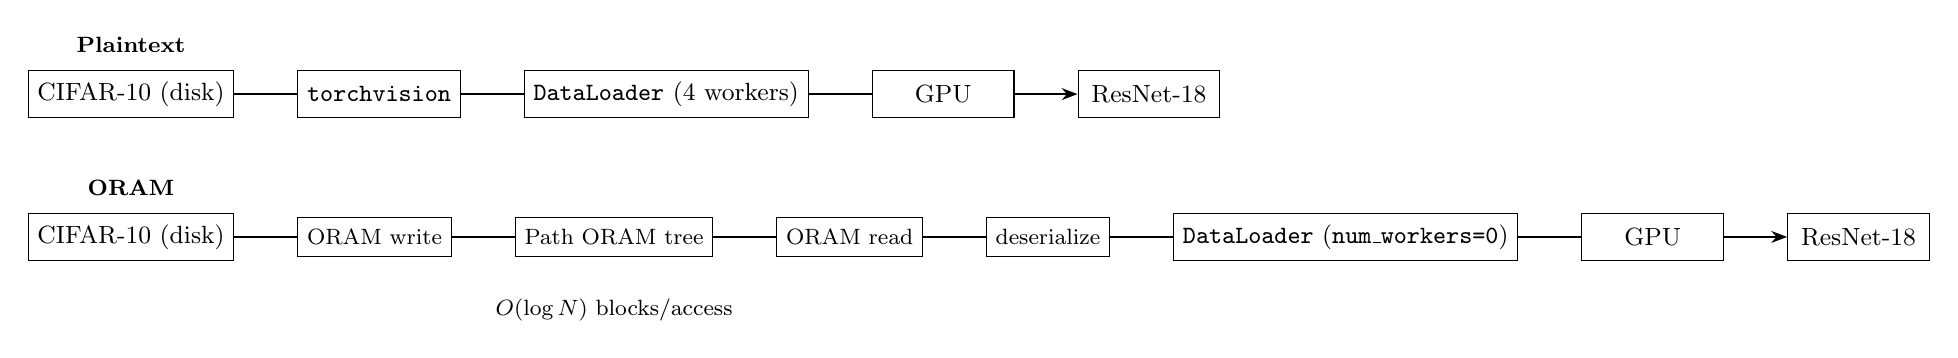
\begin{tikzpicture}[
  node distance=0.5cm and 0.8cm,
  box/.style={rectangle, draw, minimum height=0.6cm, minimum width=1.8cm, font=\small},
  smallbox/.style={rectangle, draw, minimum height=0.5cm, minimum width=1.4cm, font=\footnotesize},
  arrow/.style={-{Stealth[length=2mm]}, thick}
]
  \node[box] (disk1) {CIFAR-10 (disk)};
  \node[box, right=of disk1] (tv1) {\texttt{torchvision}};
  \node[box, right=of tv1] (dl1) {\texttt{DataLoader} (4 workers)};
  \node[box, right=of dl1] (gpu1) {GPU};
  \node[box, right=of gpu1] (model1) {ResNet-18};
  \draw[arrow] (disk1) -- (tv1) -- (dl1) -- (gpu1) -- (model1);
  \node[above=0.1cm of disk1, font=\footnotesize\bfseries] {Plaintext};

  \node[box, below=1.2cm of disk1] (disk2) {CIFAR-10 (disk)};
  \node[smallbox, right=of disk2] (write) {ORAM write};
  \node[smallbox, right=of write] (tree) {Path ORAM tree};
  \node[smallbox, right=of tree] (read) {ORAM read};
  \node[smallbox, right=of read] (deser) {deserialize};
  \node[box, right=of deser] (dl2) {\texttt{DataLoader} (\texttt{num\_workers=0})};
  \node[box, right=of dl2] (gpu2) {GPU};
  \node[box, right=of gpu2] (model2) {ResNet-18};
  \draw[arrow] (disk2) -- (write) -- (tree) -- (read) -- (deser) -- (dl2) -- (gpu2) -- (model2);
  \node[above=0.1cm of disk2, font=\footnotesize\bfseries] {ORAM};

  \node[below=0.4cm of tree, font=\footnotesize] {$O(\log N)$ blocks/access};
\end{tikzpicture}%
}
\caption{Comparison of plaintext and ORAM-backed data loading pipelines. In the ORAM-backed pipeline, logical sample accesses are mediated through randomized physical accesses, removing direct correspondence between observed storage operations and training samples.}
\label{fig:pipeline}
\end{figure}

\subsection{Storage and Serialization}

Each CIFAR-10 sample (32$\times$32$\times$3 image + 1-byte label) is serialized into a fixed-size block using \texttt{struct.pack}: a 4-byte index header, 1-byte label, and 3072-byte flattened image array, totaling 3077~bytes.
Blocks are padded to the ORAM block size (default 4096~bytes).
The block size must be at least as large as the serialized sample; smaller values are rejected at initialization.

\subsection{Single-Threaded Constraint and Mediated Loader}

PyORAM's Path ORAM requires exclusive access to the storage tree: the shared position map and client stash are not thread-safe, and concurrent eviction passes create race conditions.
This forces \texttt{num\_workers=0} in the PyTorch DataLoader, eliminating multi-worker prefetching and costing an additional ${\sim}4\times$ throughput.

To partially recover parallelism without modifying the ORAM implementation, we implemented a \emph{mediated loader}: the main thread performs all ORAM reads serially into a buffer, then wraps the pre-fetched data in a standard \texttt{Dataset} and hands it to a \texttt{DataLoader} with zero workers for CPU-bound transforms (normalization, augmentation).
This architecture separates the thread-unsafe ORAM access from the parallelizable transform stage.

%% ----------------------------------------------------------------
\section{Overhead Model}
\label{sec:model}

The total per-sample overhead can be decomposed as:
\[
\text{Overhead}_{\text{total}} \approx \underbrace{\frac{O(\log N) \times B}{S}}_{\text{I/O amplification}} \times \underbrace{C_{\text{crypto}}}_{\text{AES cost}} \times \underbrace{\frac{W_{\text{baseline}}}{W_{\text{ORAM}}}}_{\text{parallelism loss}} \times \underbrace{C_{\text{ser}}}_{\text{serialization}}
\]
where $B = 4096$ bytes is the ORAM block size, $S = 3072$ bytes is the sample size, $C_{\text{crypto}} \approx 1.5$ accounts for AES overhead, $W_{\text{baseline}} = 4$ workers, $W_{\text{ORAM}} = 1$, and $C_{\text{ser}} \approx 1.1$ accounts for \texttt{struct.pack}/\texttt{unpack} overhead.
For $N = 50{,}000$ ($h = 16$, so ${\sim}34$ block operations per access including read and write-back):
\[
\text{Overhead} \approx \frac{34 \times 4096}{3072} \times 1.5 \times 4 \times 1.1 \approx 300\times
\]
This decomposition is illustrative rather than predictive and is intended to explain observed scaling trends rather than provide a precise bound.
It assumes full tree-depth traversal on every access and no caching.
In practice, stash hits, OS page-cache effects, and AES-NI hardware acceleration reduce constant factors substantially, yielding the measured 90--180$\times$ per-epoch overhead at 50K samples (Table~\ref{tab:batch}).
The $O(\log N)$ scaling term dominates regardless of constant-factor reductions.

Table~\ref{tab:breakdown} shows the measured time distribution during ORAM training.

\begin{table}[t]
\centering
\caption{Overhead breakdown during ORAM-integrated training (ResNet-18, CIFAR-10, batch size 128, 50K samples).}
\label{tab:breakdown}
\small
\begin{tabular}{@{}lrc@{}}
\toprule
\textbf{Category} & \textbf{\% of Total} & \textbf{Source} \\
\midrule
ORAM tree operations   & 60--70\% & $O(\log N)$ block I/O + AES encrypt/decrypt \\
Forward/backward       & 15--25\% & GPU model training (unchanged) \\
Serialization          & 5--10\%  & \texttt{struct.pack}/\texttt{unpack} per sample \\
CPU$\to$GPU transfer   & 2--5\%   & Tensor copy to device \\
Batch shuffling        & $<$1\%   & Index permutation per epoch \\
\bottomrule
\end{tabular}
\end{table}

%% ----------------------------------------------------------------
\section{Experimental Evaluation}
\label{sec:eval}

Unless otherwise noted, results are intended to illustrate system-level trends and trade-offs rather than provide directly comparable performance benchmarks across differing configurations.

\subsection{Setup}

\begin{table}[t]
\centering
\caption{Default configuration. Each experiment varies one parameter from this baseline.}
\label{tab:platform}
\small
\begin{tabular}{@{}ll@{}}
\toprule
\textbf{Parameter} & \textbf{Value} \\
\midrule
Hardware      & Apple Silicon (MPS backend) \\
Framework     & PyTorch 2.x \\
ORAM          & Path ORAM via PyORAM v0.2.0~\cite{pyoram}, AES-CTR encrypted blocks \\
Model         & ResNet-18, adapted for CIFAR-10 (3$\times$3 conv1, no maxpool) \\
Dataset       & CIFAR-10 (50K train / 10K test) \\
Batch size    & 128 \\
Block size    & 4096 bytes \\
Optimizer     & SGD (lr=0.1, momentum=0.9, weight\_decay=5e-4) \\
Schedule      & MultiStepLR at epochs 50, 75, 90 ($\gamma$=0.1) \\
\bottomrule
\end{tabular}
\end{table}

ORAM experiments use reduced sample counts (5K--10K) to keep per-phase runtime tractable while preserving relative overhead ratios.
All timing measurements report wall-clock time inclusive of data-loading, compute, and optimizer steps.
Each phase uses 2--3 training epochs; the objective is steady-state throughput measurement, not convergence to final accuracy.
``Best Acc'' in all tables refers to the highest top-1 test-set accuracy observed across epochs within that phase.

\subsection{Baseline and Backend Sensitivity}
\label{sec:backend}

Plaintext training on MPS achieves ${\sim}135$\,s/epoch at 50K samples.
File-backed ORAM at 10K samples runs at ${\sim}56$\,s/epoch (Table~\ref{tab:backend}).

Replacing the file backend with in-memory storage eliminates filesystem syscalls on the ORAM tree.

\begin{table}[t]
\centering
\caption{Backend comparison (10K samples, 2 epochs, 4\,KB blocks). Similar performance across backends suggests ORAM access overhead dominates backend latency differences under this configuration.}
\label{tab:backend}
\small
\begin{tabular}{@{}lcc@{}}
\toprule
\textbf{Backend} & \textbf{Total Time (s)} & \textbf{Best Acc (\%)} \\
\midrule
File  & 112.9 & 35.78 \\
RAM   & 94.6  & 39.80 \\
\bottomrule
\end{tabular}
\end{table}

\begin{figure}[t]
\centering

\includegraphics[width=0.65\linewidth]{results/figures/fig1_backend_sensitivity.png}
\caption{Epoch time by storage backend. RAM reduces total time by 16\%.}
\label{fig:backend}
\end{figure}

The RAM backend reduces total time by 16\% (112.9\,s $\to$ 94.6\,s), bounding the contribution of filesystem overhead: page-cache misses, VFS path resolution, and journal writes account for at most 16\% of ORAM epoch time.
The remaining 84\% is AES encryption/decryption, position-map lookups, stash management, and tree traversal.
These results indicate that backend improvements alone are insufficient to significantly reduce ORAM overhead.
Storage-layer optimizations (faster SSDs, direct I/O, io\_uring) would yield diminishing returns; reducing tree operations per logical access is a more promising direction.

\subsection{Worker Scaling}

\begin{table}[t]
\centering
\caption{Worker scaling with mediated loader (file ORAM, 10K samples, 2 epochs). Increasing workers does not yield proportional speedup, suggesting serialization in the ORAM-mediated path limits effective parallelism.}
\label{tab:workers}
\small
\begin{tabular}{@{}rcc@{}}
\toprule
\textbf{Workers} & \textbf{Total Time (s)} & \textbf{Best Acc (\%)} \\
\midrule
0 & 101.3 & 25.28 \\
1 & 98.7  & 29.56 \\
2 & 110.6 & 24.02 \\
4 & 128.3 & 30.40 \\
\bottomrule
\end{tabular}
\end{table}

\begin{figure}[t]
\centering

\includegraphics[width=0.65\linewidth]{results/figures/fig2_worker_scaling.png}
\caption{Epoch time vs.\ DataLoader workers with mediated ORAM loading.}
\label{fig:workers}
\end{figure}

Adding workers beyond 1 \emph{increases} total time.
The main-thread ORAM read phase is the critical path; additional workers add IPC overhead (socket round-trips, shared-memory copies) exceeding the benefit of parallelizing transforms on 32$\times$32$\times$3 images.
CIFAR-10 transforms take ${<}0.05$\,ms per sample, negligible relative to the ${\sim}0.4$\,ms ORAM read.
These results suggest, but do not conclusively establish, that serialization in the ORAM access path limits effective parallelism.

This result is specific to small-image datasets.
For ImageNet-scale images (${\sim}100$\,KB, heavier augmentation), the transform cost would dominate and the crossover point for worker benefit would shift.
Regardless, the mediated architecture cannot reduce the ORAM read phase; recovering that parallelism requires concurrent ORAM at the tree level~\cite{talur2026}.

\subsection{Block-Size Sweep}

The overhead model predicts per-access cost proportional to $O(\log N) \times B / S$.
Increasing $B$ increases bytes moved per tree-path traversal; decreasing $B$ below $S$ is infeasible without multi-block sample fragmentation.

\begin{table}[t]
\centering
\caption{Block-size sweep (file ORAM, 10K samples, 2 epochs). This reflects a trade-off between block I/O volume and tree height rather than a universally optimal setting.}
\label{tab:blocksize}
\small
\begin{tabular}{@{}rcc@{}}
\toprule
\textbf{Block Size (bytes)} & \textbf{Total Time (s)} & \textbf{Best Acc (\%)} \\
\midrule
4,096  & 87.0  & 35.25 \\
8,192  & 122.4 & 33.69 \\
16,384 & 117.8 & 29.81 \\
32,768 & 179.2 & 30.40 \\
65,536 & 200.9 & 30.25 \\
\bottomrule
\end{tabular}
\end{table}

\begin{figure}[t]
\centering

\includegraphics[width=0.65\linewidth]{results/figures/fig3_block_size.png}
\caption{Epoch time vs.\ ORAM block size. Monotone scaling from 4\,KB to 64\,KB.}
\label{fig:blocksize}
\end{figure}

Cost increases monotonically from 87\,s at 4\,KB to 201\,s at 64\,KB (2.3$\times$).
The 16$\times$ block-size increase does not produce a 16$\times$ cost increase because larger blocks reduce tree height and AES operates on fixed-size blocks internally.
The 8\,KB $\to$ 16\,KB anomaly (slight decrease) is within measurement noise and may reflect page-alignment effects.

The practical rule: set block size to the smallest power-of-2 fitting a single sample.
For CIFAR-10 (3,077 bytes serialized), that is 4,096 bytes.

\subsection{Model and Dataset Scaling}

\subsubsection{Model scaling.}
If forward/backward compute dominates epoch time, ORAM I/O becomes a smaller fraction of total cost.

\begin{table}[t]
\centering
\caption{Model scaling (plaintext: 50K samples, 3 epochs; ORAM: 5K samples, 2 epochs, file-backed). Results are not directly comparable across columns due to differing sample counts and epoch counts; the table shows relative compute cost across architectures within each configuration.}
\label{tab:model}
\small
\begin{tabular}{@{}lrr@{}}
\toprule
\textbf{Model} & \textbf{Plaintext (s)} & \textbf{ORAM (s)} \\
\midrule
ResNet-18        & 455.3  & 54.6  \\
ResNet-50        & 1322.7 & 150.7 \\
EfficientNet-B0  & 307.1  & 60.6  \\
\bottomrule
\end{tabular}
\end{table}

\begin{figure}[t]
\centering

\includegraphics[width=0.65\linewidth]{results/figures/fig4_model_scaling.png}
\caption{Plaintext vs.\ ORAM epoch time across model architectures.}
\label{fig:model}
\end{figure}

ResNet-50's per-sample ORAM time is 2.7$\times$ higher than ResNet-18, but its forward/backward pass is ${\sim}6\times$ more expensive.
The ORAM I/O component is constant across models (same dataset, block size, tree); the per-sample difference is entirely compute.
At higher compute-to-I/O ratios, ORAM overhead becomes a smaller fraction of total training time.

EfficientNet-B0 is faster than ResNet-18 in plaintext (depthwise separable convolutions) but comparable under ORAM, because both are I/O-bound at the ORAM data-loading rate for 5K samples.

\subsubsection{Dataset-size scaling.}
Path ORAM's per-access cost is $O(\log N)$: each access traverses a path of height $h = \lceil \log_2 N \rceil$.
Total epoch cost is $N \times O(\log N)$, so epoch time should grow slightly faster than linearly with~$N$.

\begin{table}[t]
\centering
\caption{Training time as a function of dataset size (2 epochs, file-backed ORAM). Results show non-linear scaling due to ORAM access overhead and system-level effects. The 25K sample result is treated as an outlier and excluded from trend interpretation.}
\label{tab:dataset}
\small
\begin{tabular}{@{}rrr@{}}
\toprule
\textbf{$N$} & \textbf{Total Time (s)} & \textbf{Best Acc (\%)} \\
\midrule
5,000   & 96.4    & 26.25 \\
10,000  & 159.6   & 29.76 \\
25,000  & 1,537.6$^\dagger$ & 42.42 \\
50,000  & 469.1   & 56.60 \\
\bottomrule
\end{tabular}
\vspace{1pt}
{\footnotesize $^\dagger$Non-representative single-run anomaly; excluded from conclusions.}
\end{table}

\begin{figure}[t]
\centering

\includegraphics[width=0.65\linewidth]{results/figures/fig5_dataset_scaling.png}
\caption{Epoch time vs.\ dataset size for ORAM-backed training. The N=25,000 outlier is excluded from trend interpretation.}
\label{fig:dataset}
\end{figure}

The 5K$\to$10K transition shows 1.66$\times$ time increase for 2$\times$ sample increase, consistent with one additional tree level adding ${\sim}7$\% per-access cost atop the linear sample-count factor.

Training time increases with dataset size, though scaling is not strictly linear.
The 25K-sample result is an outlier and is treated as non-representative; it is not used to support conclusions about scaling behavior.

\subsection{Batch-Size Sensitivity}

\begin{table}[t]
\centering
\caption{Batch-size sweep (plaintext: 50K samples, 3 epochs; ORAM: 5K samples, 2 epochs, file-backed). Times reflect different sample counts and are not directly comparable; the table shows batch-size sensitivity within each configuration.}
\label{tab:batch}
\small
\begin{tabular}{@{}rrr@{}}
\toprule
\textbf{Batch Size} & \textbf{Plaintext (s)} & \textbf{ORAM (s)} \\
\midrule
32  & 698.0 & 86.4 \\
64  & 677.5 & 54.9 \\
128 & 451.4 & 52.3 \\
256 & 416.0 & 51.5 \\
512 & 440.8 & 51.8 \\
\bottomrule
\end{tabular}
\end{table}

\begin{figure}[t]
\centering

\includegraphics[width=0.65\linewidth]{results/figures/fig6_batch_size.png}
\caption{Epoch time vs.\ batch size for plaintext and ORAM training.}
\label{fig:batch}
\end{figure}

ORAM epoch time is stable across batch sizes 64--512 (${\sim}51$--55\,s at 5K samples).
Per-sample ORAM I/O cost is independent of batch size: each \texttt{\_\_getitem\_\_(i)} call traverses the tree regardless of batch composition.
The batch=32 outlier (86.4\,s) reflects higher per-batch overhead from more frequent optimizer steps.
Larger batch sizes amortize some per-sample overhead but do not eliminate ORAM access costs.

Plaintext training benefits from larger batches due to better GPU kernel utilization.
The 90--180$\times$ per-epoch overhead range (reported in the abstract) reflects the full 50K-sample, file-backed configuration.
At 5K samples, tree height is reduced ($h{=}13$ vs.\ $h{=}16$), cutting per-access I/O by ${\sim}19$\%; GPU acceleration on MPS reduces the compute baseline relative to CPU-only training; and warm filesystem caches from sequential phase execution reduce file-backend latency.
The theoretical upper bound of ${\sim}300\times$ (\S\ref{sec:model}) assumes worst-case traversal depth and no caching; practical constant-factor reductions account for the gap.

\subsection{Access-Pattern Leakage}

\begin{figure}[t]
\centering

\includegraphics[width=0.85\linewidth]{results/figures/fig7_leakage.png}
\caption{Distribution of logical access frequency under standard data shuffling. Both plaintext and ORAM-backed pipelines exhibit uniform logical access distributions; the privacy distinction arises from whether physical access patterns can be linked to logical samples, which is prevented by ORAM.}
\label{fig:leakage}
\end{figure}

Under standard uniform shuffling, both plaintext and ORAM logical access frequencies are approximately uniform.
The privacy distinction is in the \emph{physical} access pattern.
The histogram reflects logical access frequency; the privacy benefit of ORAM arises from obfuscatedcation of the mapping between logical and physical accesses, rather than changes in logical distribution.

In plaintext training, each logical access maps to a single deterministic address under the modeled setup.
An adversary monitoring the storage layer can observe which sample was read and in what order, enabling reconstruction of the full epoch permutation.
Under curriculum learning or data-dependent sampling, the frequency distribution becomes skewed, making observable which samples are accessed more frequently.

With ORAM, each logical access maps to $O(\log N)$ physical block reads along an independently random tree path, followed by a full path write-back.
Path ORAM constructions aim to make the physical access sequence computationally indistinguishable for any two equal-length logical access sequences~\cite{stefanov2013}.
The empirical results illustrate that the implemented ORAM-backed loader removes the direct linkage between observed physical accesses and logical samples.

\subsection{Combined Optimization}

The individual-phase results suggest RAM backend and 4\,KB blocks as optimal, while worker scaling shows \texttt{num\_workers=0} is best for CIFAR-10.
To test whether combining RAM backend with multi-worker loading yields a net benefit, we evaluate a combined configuration.

\begin{table}[t]
\centering
\caption{Interaction of backend and worker configuration (ResNet-18, CIFAR-10, 10K ORAM samples). Results are not directly comparable due to differing sample counts; the table shows relative behavior within each configuration.}
\label{tab:combined}
\small
\begin{tabular}{@{}lccc@{}}
\toprule
\textbf{Configuration} & \textbf{Epochs} & \textbf{Total (s)} & \textbf{Best Acc (\%)} \\
\midrule
Plaintext (50K, 4 workers)       & 3 & 409.6 & 50.15 \\
ORAM baseline (file, \texttt{num\_workers=0})        & 2 & 84.8  & 29.04 \\
ORAM combined (ram, \texttt{num\_workers=4})         & 2 & 144.2 & 25.49 \\
\bottomrule
\end{tabular}
\end{table}

The combined RAM + multi-worker configuration is slower (144.2\,s vs.\ 84.8\,s), confirming that multi-worker IPC cost dominates any benefit from the RAM backend for this image size.
The best-performing ORAM configuration for CIFAR-10 under the tested conditions is: RAM backend, \texttt{num\_workers=0}, 4\,KB blocks---combining the RAM backend's 16\% improvement (\S\ref{sec:backend}) with zero-worker loading to avoid IPC overhead.

%% ----------------------------------------------------------------
\section{Membership Inference Signal Demonstration}
\label{sec:inference}

To illustrate that access patterns can provide signal for downstream privacy attacks, we conduct a simple membership inference demonstration using access frequency as the sole feature.

\subsection{Setup}

We split CIFAR-10 into two disjoint sets: a training set (20K samples) used for model training, and a holdout set (20K samples) never accessed during training.
This setup represents an upper-bound signal scenario where holdout samples are never accessed, producing a binary access pattern.
We train a simple CNN for 3 epochs using standard PyTorch data loading with shuffling enabled, logging the access count for each sample.
After training, we use access frequency as a feature to distinguish training samples from holdout samples.

\subsection{Attack Model}

We train a logistic regression classifier using access count as the single feature.
The intuition is straightforward: training samples are accessed multiple times per epoch (3 epochs $\times$ expected frequency $\approx$ 3 accesses per sample), while holdout samples are never accessed (access count = 0).
This is an intentionally simple attack that does not represent state-of-the-art membership inference techniques, but demonstrates that access frequency alone provides a measurable signal.

\subsection{Results}

\begin{table}[t]
\centering
\small
\caption{Membership inference performance using access frequency as the sole feature. Plaintext training enables near-perfect separation due to deterministic access logging in this controlled setup (accessed vs.\ never accessed); ORAM-backed training prevents construction of per-sample access counts.}
\label{tab:membership}
\begin{tabular}{lcc}
\toprule
\textbf{Setting} & \textbf{Accuracy} & \textbf{AUC} \\
\midrule
Plaintext & 1.00 & 1.00 \\
ORAM-backed & N/A & N/A \\
\bottomrule
\end{tabular}
\end{table}

\begin{figure}[t]
\centering

\includegraphics[width=0.75\linewidth]{results/figures/membership_auc.png}
\caption{Access count distribution for training vs.\ holdout samples. Training samples exhibit non-zero access counts, while holdout samples have zero accesses, enabling perfect membership classification in the plaintext setting. Under ORAM, physical accesses cannot be linked to logical samples, preventing construction of per-sample access counts.}
\label{fig:membership}
\end{figure}

Table~\ref{tab:membership} and Figure~\ref{fig:membership} show the results.
In the plaintext setting, the attack achieves perfect separation (AUC = 1.00) because training samples have non-zero access counts while holdout samples have zero accesses.
This result reflects the deterministic nature of access logging in plaintext training rather than a sophisticated attack: any threshold $\tau > 0$ achieves perfect classification.

In the ORAM-backed setting, physical accesses are randomized and unlinkable to logical samples.
An adversary observing physical block accesses cannot construct per-sample access counts, rendering the attack infeasible.
The attack model assumes access to per-sample access frequencies, which ORAM removes by design.

\subsection{Discussion}

This demonstration is intentionally simple and does not constitute a full membership inference evaluation.
The attack relies on statistical differences in access patterns (accessed vs.\ never accessed) rather than binary visibility alone.
It shows that access frequency alone provides a strong signal for membership classification when access patterns are directly observable, and that ORAM mitigates this signal by removing the correspondence between observed physical accesses and logical samples.

The perfect separation (AUC = 1.00) reflects the binary nature of the setup (accessed vs.\ never accessed) rather than a sophisticated attack.
More realistic scenarios with partial dataset overlap, data augmentation, or non-uniform sampling would produce weaker but still meaningful signals.
This result demonstrates that access-pattern exposure can provide usable signal for downstream membership inference under the modeled threat model.

%% ----------------------------------------------------------------
\section{Discussion and Limitations}
\label{sec:limitations}

The dominant finding is that ORAM overhead is intrinsic to the cryptographic protocol, not the storage medium.
The 16\% backend improvement sets an upper bound on what storage-layer engineering can achieve; the remaining 84\% requires algorithmic improvements such as concurrent ORAM, reduced tree depth, or batched eviction.

The mediated multi-worker architecture does not benefit small images because IPC overhead exceeds transform cost.
For larger images with heavier augmentation pipelines, the crossover point should shift in favor of workers.

More broadly, these results characterize access-pattern leakage as a meaningful and under-addressed privacy channel in ML systems, outside the scope of data privacy and gradient privacy protections.
We empirically demonstrate that access frequency alone provides a measurable signal for membership inference (Section~\ref{sec:inference}).
Existing defenses (federated learning, differential privacy, secure enclaves) do not address the storage access channel; an adversary with visibility into storage I/O metadata can observe training access behavior without ever observing a data value or a gradient.

\medskip
\noindent\textbf{Scope limitations.}
(1)~All phases use 2--3 epochs; accuracy values reflect early training, not converged model quality.
(2)~CIFAR-10's 32$\times$32 images fit in a single 4\,KB block; larger images would change block-size dynamics and the worker-scaling crossover.
(3)~MPS-only hardware; CUDA GPUs with different memory bandwidth ratios may produce different profiles.
(4)~The $N{=}25{,}000$ anomaly requires controlled memory-pressure investigation.
(5)~Batch-index shuffling uses standard \texttt{numpy} shuffle, not an oblivious protocol~\cite{ngai2024}; batch composition remains visible.
(6)~ORAM does not hide dataset size; concealing capacity requires padding to a fixed tree size.

%% ----------------------------------------------------------------
\section{Conclusion and Future Work}

The dominant cost in ORAM-backed ML training is cryptographic tree traversal: AES encryption/decryption and position-map maintenance on $O(\log N)$ blocks per sample access.
Storage backend optimization (file $\to$ RAM) yields a bounded 16\% improvement; the remaining overhead is intrinsic to Path ORAM.
Data-loader-level parallelism cannot compensate for single-threaded ORAM access when per-sample transform cost is small relative to per-sample ORAM read cost.

Block size should be set to the minimum fitting a single sample.
Compute-heavy models reduce the relative contribution of ORAM I/O.
Per-access cost scales logarithmically with dataset size, consistent with Path ORAM's theoretical bound.
The ORAM data-loading layer is intended not to alter model semantics: it delivers the same logical sample sequence to the training loop, preserving the data stream seen by the model while removing the direct correspondence between logical sample accesses and observed physical block accesses.

We do not evaluate advanced or state-of-the-art membership inference attacks, but demonstrate that access frequency alone provides a measurable signal for membership inference under the modeled setup.
We do not evaluate label inference or attribute recovery attacks.

These findings highlight the importance of considering access-pattern leakage in observable ML systems.
Storage-level access patterns represent a distinct attack surface that is not addressed by existing model- and gradient-level privacy mechanisms.

\medskip
\noindent\textbf{Future work.}
(1)~Integrating concurrent ORAM such as SONIC~\cite{talur2026} to recover multi-worker parallelism.
(2)~Replacing standard shuffle with oblivious random permutation~\cite{ngai2024} to obscure batch composition.
(3)~Moving AES operations to the GPU to overlap cryptographic and compute workloads.
(4)~Extending evaluation to ImageNet-scale images and Vision Transformers to characterize overhead at higher compute-to-I/O ratios and multi-block samples.
(5)~Evaluating the system with comprehensive membership inference attacks using richer access-pattern features and partial observability.

\medskip
\noindent\textbf{Reproducibility.}
We will release code and scripts to reproduce all experiments upon publication.

%% ----------------------------------------------------------------
\begin{thebibliography}{15}

\bibitem{goldreich1996}
Goldreich, O., Ostrovsky, R.:
Software protection and simulation on oblivious RAMs.
J.~ACM \textbf{43}(3), 431--473 (1996)

\bibitem{stefanov2013}
Stefanov, E., van Dijk, M., Shi, E., Fletcher, C., Ren, L., Yu, X., Devadas, S.:
Path ORAM: An extremely simple oblivious RAM protocol.
In: Proc.\ ACM CCS, pp.~299--310 (2013)

\bibitem{talur2026}
Talur, A., Demertzis, I.:
SONIC: Concurrent oblivious RAM.
In: Proc.\ USENIX Security (to appear, 2026)

\bibitem{mavrogiannakis2025}
Mavrogiannakis, A., et~al.:
OBLIVIATOR: Oblivious parallel operators for secure database joins.
In: Proc.\ USENIX Security (2025)

\bibitem{ngai2024}
Ngai, B., et~al.:
Distributed and scalable oblivious sorting and shuffling.
In: Proc.\ IEEE S\&P (2024)

\bibitem{pyoram}
Hackebeil, G.:
PyORAM: Python ORAM implementation (v0.2.0).
\url{https://github.com/ghackebeil/PyORAM} (accessed Mar.\ 2026)

\bibitem{dwork2006}
Dwork, C., McSherry, F., Nissim, K., Smith, A.:
Calibrating noise to sensitivity in private data analysis.
In: Proc.\ TCC, pp.~265--284 (2006)

\bibitem{mcmahan2017}
McMahan, B., Moore, E., Ramage, D., Hampson, S., y~Arcas, B.A.:
Communication-efficient learning of deep networks from decentralized data.
In: Proc.\ AISTATS, pp.~1273--1282 (2017)

\bibitem{shokri2017}
Shokri, R., Stronati, M., Song, C., Shmatikov, V.:
Membership inference attacks against machine learning models.
In: Proc.\ IEEE S\&P, pp.~3--18 (2017)

\bibitem{xu2015}
Xu, Y., Cui, W., Peinado, M.:
Controlled-channel attacks: Deterministic side channels for untrusted operating systems.
In: Proc.\ IEEE S\&P, pp.~640--656 (2015)

\bibitem{tramer2019}
Tram\`{e}r, F., Boneh, D.:
Slalom: Fast, verifiable and private execution of neural networks in trusted hardware.
In: Proc.\ ICLR (2019)

\bibitem{juvekar2018}
Juvekar, C., Vaikuntanathan, V., Chandrakasan, A.:
GAZELLE: A low latency framework for secure neural network inference.
In: Proc.\ USENIX Security, pp.~1651--1669 (2018)

\bibitem{yan2020}
Yan, M., Fletcher, C., Torrellas, J.:
Cache telepathy: Leveraging shared resource attacks to learn DNN architectures.
In: Proc.\ USENIX Security, pp.~2003--2020 (2020)

\bibitem{bonawitz2017}
Bonawitz, K., et~al.:
Practical secure aggregation for privacy-preserving machine learning.
In: Proc.\ ACM CCS, pp.~1175--1191 (2017)

\bibitem{gramine2022}
Tsai, C.-C., et~al.:
Gramine: A library OS for unmodified applications on SGX.
In: Proc.\ USENIX ATC (2022)

\end{thebibliography}

\end{document}
